
\section{组合数的两个性质}
\begin{thm}{定理1}
\[\comb{n}{m}=\comb{n}{n-m}\]
\end{thm}

\begin{proof}
$\because\quad \comb{n}{m}=\frac{n!}{m!(n-m)!}$,

$\comb{n}{n-m}=\frac{n!}{(n-m)![n-(n-m)]!}=\frac{n!}{m!(n-m)!}$

$\therefore\quad \comb{n}{m}=\comb{n}{n-m}.$
\end{proof}



这个性质也可以根据组合的定义得出：从$n$个不同元素中取出$m$个元素后，剩下 $(n-m)$ 个元素，也就是说，从$n$个不同元素中取出$m$个元素的每一个组合，都对应着从$n$个不同元素中取出剩下的 $(n-m)$ 个元素的唯一的一个组合；反过来也是一样。因此，从$n$个不同元素中取出$m$个元素的组合数$\comb{n}{m}$，于从$n$个不同元素中取出$( n-m )$个元素的组合数$\comb{n}{n-m}$，即
\[\comb{n}{m}=\comb{n}{n-m}.\]

当$m>\frac{n}{2}$时，通常我们不直接计算$\comb{n}{m}$，而是改为计算
$\comb{n}{n-m}$，这样比较简便。例如，$\comb{10}{8}$ 可以这样计算：
\[\comb{10}{8}=\comb{10}{10-8}=\comb{10}{2}=\frac{10\x 9}{1\x 2}=45\]

\begin{remark}
    为了使这个公式在$n=m$ 时也成立，我们规定
\[\comb{n}{0}=1.\]
\end{remark}

\begin{thm}{定理2}
\[
\comb{n+1}{m}=\comb{n}{m}+\comb{n}{m-1}
 \]   
\end{thm}

\begin{proof}
\[\begin{split}
    \comb{n}{m}+\comb{n}{m-1}&=\frac{n!}{m!(n-m)!}+\frac{n!}{(m-1)!(n-m+1)!}\\
&=\frac{n!(n-m+1)+n!m}{m!(n-m+1)!}\\
&=\frac{(n-m+1+n)n!}{m!(n-m+1)!}\\
&=\frac{(n+1)!}{m![(n+1)-m]!}\\
&=\comb{n+1}{m}
\end{split}\]

$\therefore\quad \comb{n+1}{m}=\comb{n}{m}+\comb{n}{m-1}$
\end{proof}


这个性质也可以根据组合的定义和加法原理得出。从$a_{1},a_{2},\ldots,a_{n+1}$ 这$( n+1 )$个不同的元素中取出$m$个的组合数是$\comb{n+1}{m}$，这些组合可以分成两类，一类含有$a_{1}$，一类不含$a_{1}$, 含有$a_{1}$的组合是从$a_{2},a_{3},\ldots,a_{n+1}$ 这$n$个元素中取出$( m-1 )$个元素与$a_{1}$ 组合的，共有$\comb{n}{m-1}$ 个；不含$a_{1}$ 的组合是$a_{2},a_{3},\ldots,  a_{n+1}$ 这$n$个元素中取出$m$个元素组成的，共有$\comb{n}{m}$ 个。根据加法原理，得
\[\comb{n+1}{m}=\comb{n}{m}+\comb{n}{m-1}\]

\begin{example}
    计算：
\begin{enumerate}[(1)]
    \item $\comb{200}{197}$;
\item $\comb{1}{4}+\comb{7}{6}$.
\end{enumerate}
\end{example}

\begin{solution}
\begin{enumerate}[(1)]
\item 由定理1，得
\[
\comb{200}{197}=\comb{200}{200-197}=\comb{200}{3}=\frac{200\x  199\x  198}{1\x  2\x  3}=1313400;
\]
    \item 由定理2，得
\[
\comb{7}{4}+\comb{7}{8}=\comb{8}{4}=\frac{8\x  7\x  6\x  5}{1\x  2\x  3\x  4}=70.\]
\end{enumerate}
\end{solution}
    
\begin{example}
    计算：$ \comb{2n}{12-n}+\comb{4+n}{2n}$
\end{example}

\begin{analyze}
    为确定其和的结果，需先确定$n$。由组合数公式，有
\[\begin{cases}
    2n\ge  12-n,\\
    4+n\ge  2n.
\end{cases}\]
解得$4\le  n\le  4$，即$n=4$.

$\therefore\quad \comb{2n}{12-n}+\comb{4+n}{2n}=\comb{8}{8}+\comb{8}{8}=2$.
\end{analyze}

\begin{example}
    甲有7本不同的数学书，乙有9本不同的物理书，互相交换两本书，有多少种交换方法？
\end{example}

\begin{analyze}
    甲从7本不同的数学书中取出两本，这两本是不管顺序的，所以共有$ \comb{7}{2} $种取法；同理，乙从9本不同的物理书中取出两本，也是无序的，共有$ \comb{9}{2} $种取法。要完成交换这件事，需分两步走。第一步，甲取出两本书；第二步，乙取出两本书，进行交换无顺序问题，所以应用乘法原即可解决。
\end{analyze}

\begin{solution}
根据题意，甲需取出2本数学书，应有$ \comb{7}{2} $种取法；乙需取出2本物理书，应有$ \comb{9}{2} $种取法。由乘法原理，有
\[
\comb{7}{2}\cdot  \comb{9}{3}=\frac{7\x  6}{2\x  1}\cdot \frac{9\x  8}{2\x  1}=756.\]

答：共有756种交换方法。    
\end{solution}

\begin{example}
    在产品检验时，常从产品中抽出一部分进行检查。现在从100件产品中任意抽出3件：
\begin{enumerate}[(1)]
    \item 一共有多少种不同的抽法？
    \item 如果100件产品中有2件次品，抽出的3件中恰好有1件是次品的抽法有多少种？
    \item 如果100件产品中有2件次品，抽出的3件至少有 1件是次品的抽法是有少种？
\end{enumerate}
\end{example}

\begin{analyze}
\begin{enumerate}[(1)]
   \item 从产品中任意抽出3件，因为不必管这3件的顺序，所以是组合问题。
   \item 欲使“抽出的3件产品中恰有一件次品”这件事完成，需分两步。第一步，从两件次品中任意抽出一件；第二步，从$(100-2)$种正品中任意抽出两件。
\item 欲使“抽出的3件产品中至少有1件次品”这件事完成可以分两类：“抽出的3件中有1件次品”，“抽出的3件中有 2件次品”。可分别计算这两类的取法的种数，然后用加法原理。

此问也可用间接求法，先求出从100件产品中任取出3件的总数，再减去取出的3件产品全是合格产品的抽法总数。
\end{enumerate}
\end{analyze}

\begin{solution}
\begin{enumerate}[(1)]
    \item 所求的不同抽法的种数，就是从100件产品中取出3件的组合数：
\[
\comb{100}{3}=\frac{100\x  99\x  98}{3\x  2\x  1}=161700.
\]

答：共有161700种抽法。    
\item 从2件次品中抽出1件次品的抽法有$ \comb{2}{1} $种，从 98件合格品中抽出2件合格品的抽法有$ \comb{2}{2} $种，因此抽出的3件中恰好有1件是次品的抽法的种数是
\[
\comb{2}{1}\cdot  \comb{98}{2}=2\x  4753=9506.\]

答：3件中恰好有1件是次品的抽法有9506种。

\item \textbf{解法1：}由(2)，3件中恰好有1件是次品的抽法有$ \comb{2}{1}\cdot  \comb{98}{2} $种，同理，抽出3件产品，恰好有2件是次品的抽法有 $\comb{3}{2}\cdot  \comb{91}{1} $种。因此抽出的3件中至少有一件是次品的抽法种数是
\[
\comb{2}{1}\cdot  \comb{98}{2}+\comb{2}{2}\cdot  \comb{98}{1}=9506+98=9604.\]

\textbf{解法2：}从100件产品中抽出3件，一共有$ \comb{100}{3} $种抽法，在这些抽法中，除掉抽出的3件都是合格品的抽法$ \comb{98}{3} $种，使得到抽出的3件中至少有1件是次品的抽法的种数，即
\[
\comb{100}{3}-\comb{98}{3}=161700-152096=9604.\]

答：3件中至少有1件是次品的抽法有9604种。
\end{enumerate}
\end{solution}

\begin{rmk}
\begin{enumerate}
    \item 第(3)小题的上述两种解法，解法2不需要细致分类，这种间接解法往往较直接，解法易于思考。
    \item 第(3)小题是否可以这样来解：
\end{enumerate}

从100件产品抽出的3件中至少有1件是次品的抽法，可以先从次品中抽出1件，然后再从余下的99件产品中任抽出2件，这样就保证了至少有1件次品。

这种解法得到的答案是$ \comb{2}{1}\cdot  \comb{99}{2}=9702$. 比前面解法多出98种。错误出在哪里？这里由于先取出的一件次品若是次品甲，在取剩下99件中的2件产品时，可能把次品乙和正品$a$取出，若先取出的一件次品是次品乙，而后取出的2件产品恰好是次品甲与正品$a$时，这两种取法显然是同一种取法，只是次品甲、乙取出次序不同。因而，这种解法实际上会出现重复的组合，种数当然比正确答案要多。
\end{rmk}

\begin{example}
    平面内有9个点，其中4个点在一直线上，此外没有三点共线。
\begin{enumerate}[(1)]
    \item 过其中任意两点作一直线，一共可以作出多少条直线？
    \item 以其中三点为顶点，可以作出多少个三角形？
\end{enumerate}
\end{example}

\begin{analyze}
    本题是“有条件限制”（4个点共线）的组合问题。这里由于受限制的元素（点）太多，用直接解法就要对受限制的元素分类，那将很复杂，所以可用间接解法，便于思考。
\end{analyze}

\begin{solution}
\begin{enumerate}[(1)]
    \item 若不考虑“其中4个点在一直线上”这一条件，所求直线的条数是从9个不同元素中取出2个元素的组合数，可作出$ \comb{9}{2} $条直线。但由于4个点在一直线上，其中有$ \comb{4}{2} $条直线重合成一条直线，应在总数中除去重合的条数。因此可以作出直线的条数为
\[
\comb{9}{2}-\comb{4}{2}+1=31.\]

答：可以作出31条直线。

\item 从9个点中，取出3个点可以作出$ \comb{9}{3} $个三角形。但由于4个点在一条直线上，若取出的3个点全在这4个点之中，则不能作出三角形，也就是说有 $\comb{4}{3} $个三角形实际上是作不出来的。因此共可以作出三角形的个数为
\[
\comb{9}{3}-\comb{4}{3}=80.\]

答：可以作出80个三角形。


\end{enumerate}
\end{solution}


\begin{example}
     有11个工人，其中5人只能当木工，4人只能当瓦工，2人既能当木工又能当瓦工，现要从11人中选出4个木工和 4个瓦工组成一个工程队，共有多少种分配方案？
\end{example}

\begin{analyze}
    本题中“完成一件事”就是“从11人中选出4个木工和4个瓦工”，要做完这件事可分两步，第一步可先选木工4人，第二步，选瓦工4人。

做第一步（选木工4人）有哪些方法呢？这里有两个集合的元素可供选择，即只会木工的5人集合，和既会木工也会瓦工的2人集合。为了找到所有的选法就要对这两个集合中的一个进行分类。一般对元素较少的集合进行分类比较简单。

所以做第一步（选木工4人）可以对既会木工又会瓦工的2人集合分类（挑选木工2人）。可有三种情况：一个都不要；只要1人；2人全要。在这样的分类下，就可得到完成第一步（选木工4人）的所有选法。当第一步完成后再做第二步。
\end{analyze}

\begin{solution}
 先从木工、瓦工均会的2人集合中挑选木工工人。若一个都不要，只好再从木工工人集合挑出4名工人；这样木工工人选好，再选瓦工。这时所余会瓦工的工人共有$4+ 2=6$ 名，再从中选4人，这样共有$ \comb{2}{0}\cdot  \comb{5}{4}\cdot  \comb{6}{4} $种选法。其他两种情况同样处理，分别有$ \comb{2}{1}\cdot  \comb{5}{3}\cdot  \comb{5}{4} $种选法和$ \comb{2}{2}\cdot  \comb{5}{2}\cdot  \comb{4}{4} $种选法。由加法原理，有
\[
\comb{2}{0}\cdot  \comb{5}{4}\cdot  \comb{6}{4}+\comb{2}{1}\cdot  \comb{5}{3}\cdot  \comb{5}{4}+\comb{2}{2}\cdot  \comb{5}{2}\cdot  \comb{4}{4}=75+100+10=185.\]

答：共有185种分配方案。   
\end{solution}

\begin{example}
    学校要从8个班中选10名同学去参加夏令营，每班至少1名，现在学校把这10个名额分配到8个班去，有多少种不同的分配方案。
\end{example}

\textbf{分析1：}“完成一件事”在这里就是完成一个分配方案，因为要求每班至少一人，所以先每班分配一个名额。这样就只剩下两个名额了，这两个名额的一种分法就对应一种分配方案。这两个名额分配情况只有两类：
\begin{enumerate}[(1)]
    \item 全部分给一个班；
    \item 分给两个班，每班一名。
\end{enumerate}

\textbf{解法1：}每班先给一个名额。剩下的两个名额，若全部分给一个班，有 $\comb{8}{1} $种方法；若任取两个班，每班各一名，共有$ \comb{8}{2} $种方法，由加法原理，共有分法$\comb{8}{1}+\comb{8}{2}=8+28=36$种。

\textbf{分析(2)：}假设一种分配方案已经确定，让选出的10名同学按班号（1—8）的次序自左至右站成一排，同班的要相邻，不同班的同学之间画一条线把他们隔开。这样因为有 8个班，隔开它们的线正好有7条。

可以想到，对应不同的分配方案，这7条隔线的位置不同，反之，7条隔线的任意一种划法，都对应一种分配方案。

这样的隔线具有下述特点：任意两隔线之间至少有一名学生，隔线两侧都有学生。

这样的7条隔线的划法共有多少种，就有多少种分配方案。

\textbf{解法2：}把10个"名额"排成一排，用7条隔线把他们隔开。每两条隔线之间至少有一名学生，每条隔线的两侧都要有学生。这样，隔线的一种划法就对应一种分配方案。因为有10个名额，可划线的位置只有9个，所以隔线的划分总数是
\[
\comb{9}{7}=\comb{9}{2}=36.\]

答：共有36种分配方案。

\begin{example}
    从8名运动员中选出4名组成$ 4\x  100 $米的接力队。甲不跑第一棒，乙不跑第四棒的安排方法共有多少种？
\end{example}

\begin{analyze}
本题中的“做一件事”指组成4人接力队，并安排
好谁跑第几棒。所以完成这件事需分两步：第一步，从8名运动员中选出4名组成接力队。这是组合问题。第二步，安排跑第几棒是排列问题。但是有限制条件：甲不跑第一棒，乙不跑第四棒。为了计算第二步，对第一步就要对包含不包含甲或乙进行分类。

组成接力队可分四种情况：4人中不含甲和乙；4人中含有甲，不含乙；4人中含乙，不含甲；4人中既含甲，又含乙。    
\end{analyze}

\begin{solution}
    4人接力队不包含甲和乙，共有选法$ \comb{6}{4} $种，这4人谁跑哪一棒都行。根据乘法原理，共有$ \comb{6}{4}\cdot  \perm{4}{4} $种安排方法； 4人接力队中含甲不含乙的选法有$ \comb{6}{3} $种，因为甲是特殊元素（他不跑第一棒），先安排他跑第二、第三、第四棒中的一棒，有$\perm{3}{1}$ 种方法，其余三棒由剩下的3人跑，有$ \perm{3}{3} $种方法。根据乘法原理共有$ \comb{6}{3}\cdot  \perm{3}{1}\cdot  \perm{3}{3} $种安排方法；4人接力队中含有乙，不含甲，与含甲不含乙的安排方法完全类似。所以也是有$\comb{6}{3}\cdot  \perm{3}{1}\cdot  \perm{3}{3}$ 种安排方法；4人接力队中既含甲又含乙，即已经有了两人，其余两人就从甲、乙以外的6人中选取，选取有$\comb{6}{2}$ 种。这样组成的4人接力队，先安排甲、又有两种排法，安排甲跑第四棒，其余3人排法有$\perm{3}{3}$ 种，若安排甲跑第二棒或第三棒，有$\comb{2}{1}$ 种，再安排乙，由于乙不跑第四棒，所以只有两棒可安排，有$\comb{2}{1}$ 种，最后再安排甲、乙以外的2人，有$\perm{2}{2}$ 种排法，根据乘法原理，所以这种4人接力队共有$\comb{6}{2}\cdot  \comb{1}{1}\cdot  \perm{3}{3}+\comb{6}{2}\cdot  \comb{2}{1}\cdot  \comb{2}{1}\cdot  \perm{2}{2}$ 种安排法。

根据加法原理，从8名运动员中选出4名组成$ 4\x  100 $米的接力队使甲不跑第一棒，乙不跑第四棒的安排共有
\[\comb{6}{4}\cdot  \perm{4}{4} +\comb{6}{3}\cdot  \perm{3}{1}\cdot  \perm{3}{3}+\comb{6}{3}\cdot  \perm{3}{1}\cdot  \perm{3}{3}+\comb{6}{2}\cdot  \comb{1}{1}\cdot  \perm{3}{3}+\comb{6}{2}\cdot  \comb{2}{1}\cdot  \comb{2}{1}\cdot  \perm{2}{2} =1290\;\text{（种）}\]

\end{solution}


































\section*{习题三}
\begin{center}
    \bfseries A
\end{center}

\begin{enumerate}
    \item 求证：
\begin{enumerate}[(1)]
    \item $\comb{n+1}{m}=\comb{n}{m-2}+\comb{n-1}{m}+\comb{n-1}{m-1}$;
    \item $\comb{n}{m+1}+\comb{n}{m-1}+2\comb{n}{m}=\comb{m+2}{m+1}$.
\end{enumerate}
\item 某校举行篮球单循环赛，有8个队参加，共需要举行多少场比赛？
\item 
解方程：
\begin{multicols}{2}
\begin{enumerate}[(1)]
    \item $\comb{n+3}{n-2}=4\perm{n+2}{3}$;
    \item $\comb{n}{3}+\comb{n}{2}=15\left(n^{2}-1\right)$.
\end{enumerate}
\end{multicols}

\item 圆上有10个点：
\begin{enumerate}[(1)]
    \item  过每2个点可作一条弦，一共可作多少条弦？
    \item 过每3个点可作一个圆内接三角形，一共可作多少个圆内接三角形？
\end{enumerate}

\item 
\begin{enumerate}[(1)]
    \item     凸五边形有多少条对角线？
    \item     凸$n$边形有多少条对角线？
\end{enumerate}
\item 
\begin{enumerate}[(1)]
    \item     空间有8个点，没有4个点在同一平面内，过每3个点作一个平面，一共可以作多少个平面？
    \item     空间有10个点，其中任何4点不共面，以每4个点为顶点作一个四面体，一共可作多少个四面体？
    \item 以一个正方体的顶点为顶点的四面体共有多少个？
\end{enumerate}
\item 在$1,2,3,\ldots,9$这9个自然数中，任取两个数，问
\begin{enumerate}[(1)]
    \item     两数之积是奇数的取法有多少种？
  \item     两数之积是偶数的取法有多少种？
  \item     两数之和是奇数的取法有多少种？
  \item 两数之和是偶数的取法有多少种？
\end{enumerate}
\item 从10本不同的书中，每次选出3本，一共有多少种选法？如果把每次取出的3本书分别分给甲、乙、丙3人，共有多少种分法？
\end{enumerate}


\begin{center}
    \bfseries B
\end{center}

\begin{enumerate}
 \setcounter{enumi}{8}   
 \item 某车间有7个技工，其中3人只能做车工，2人只能做钳工，2人既能做车工又能做钳工，现在要抽3个车工，2个钳工组成一个支农小分队，有多少种选法？
 \item 楼前栽一排树，其中5棵杨树，7棵柳树，若要求每两棵杨树都不能相邻，有多少种栽法？
 \item 从$1$、$3$、$5$、$7$、$9$中取3个数字，从$0$、$2$、$4$、$6$、$8$中取 2个数字，可作出多少个没有重复数字的且比70123大的五位数。
 \item 某小组有4个男生，3个女生，
\begin{enumerate}[(1)]
 \item 选出3人去完成一项工作，有多少种选法？
    \item 选出3人中至少有一个男生，有多少种选法？
    \item 选出3人担任三项不同的工作（每人一项），有多少种安排方法？
    \item 选出3人担任三项不同的工作（每人一项），又要求有且只有两名男生，有多少种安排方法？
\end{enumerate}
\end{enumerate}

\begin{center}
    \bfseries C
\end{center}

\begin{enumerate}
  \setcounter{enumi}{12}  
  \item 求证：$ \comb{m}{m}+\comb{m+1}{m}+\comb{m+2}{m}+\cdots+\comb{m+n}{m}=\comb{m+n+1}{m+1}$.

  \item 证明： $\comb{n}{m}=\comb{n-3}{m}+3\comb{n-3}{m-1}+3\comb{n-3}{m-2}+\comb{m-3}{m-3}$，根据组合的定义说明这等式的含义。
\end{enumerate}


\section*{二、二项式定理}

\section{二项式定理}

在初中我们曾学过
\[\begin{split}
(a+b)^{2}&=a^{2}+2ab+b^{2},\\
(a+b)^{3}&=a^{3}+3a^{2}b+3ab^{2}+b^{3}.    
\end{split}\]

但是对于任意$ n\in \N$, $(a+b)^{n}$的展开式是什么？这正是本节要研究的。

我们首先研究$ (a+b)^{4} $的展开式。虽然$ (a+b)^{4} $的展开式可利用$ (a+b) $与$ (a+b)^{3} $的展开式的乘积得出，但是为了认清其含有的内在规律，不妨从下面的乘积中来认识它。

\[\begin{split}
&\quad \left(a+b_{1}\right)\left(a+b_{2}\right)\left(a+b_{3}\right)\left(a+b_{4}\right)\\
&=a^{4}+\left(b_{1}+b_{2}+b_{3}+b_{4}\right)a^{3}+\left(b_{1}b_{2}+b_{1}b_{3}+b_{1}b_{4}+b_{2}b_{3}+b_{2}b_{4}+b_{3}b_{4}\right)a^{2}\\
&\qquad +\left(b_{1}b_{2}b_{3}+b_{1}b_{2}b_{4}+b_{1}b_{3}b_{4}+b_{2}b_{3}b_{4}\right)a+b_{1}b_{2}b_{3}b_{4}.    
\end{split}\]

令$b_{1}=b_{2}=b_{3}=b_{4}$，上面这个等式变为
\[\begin{split}
    (a+b)^{4}& =a^{4}+4a^{3}b+6a^{2}b^{2}+4ab^{3}+b^{4}\\ 
&=\comb{4}{0}a^{4}+\comb{4}{1}a^{3}b+\comb{4}{2}a^{2}b^{2}+\comb{4}{3}ab^{3}+\comb{4}{4}b^{4}.
\end{split}\]

这样我们可看出$ (a+b)^{4} $的展开式有以下特征：
\begin{enumerate}
    \item 展开式共有五项。
    \item 各项中的指数：$a$的指数在第一项是4，在以后的各项中依次递减1直至为零；$b$的指数在第一项是零，在以后的各项中依次递增1直至为4。展开式中的每一项中$a$与$b$的指数和为4，即展开式是关于$a$、$b$的四次齐次式。
    \item 展开式中第$( r+1 )$项的系数是$\comb{4}{r}\;   (r=0,1,2,3,4)$, 因此，展开式中各项的系数依次排列为：
\[\comb{4}{0},\quad \comb{4}{1},\quad \comb{4}{2},\quad \comb{4}{3},\quad \comb{4}{4}.\]
\end{enumerate}


一般地，对于任意$ n\in \N$，我们猜想
\[\begin{split}
(a+b)^{n}&=\comb{n}{0}a^{n}+\comb{n}{1}a^{n-1}b+\comb{n}{2}a^{n-2}b^{2}+\cdots\\
& \qquad +\comb{n}{r}a^{n-r}b^{r}+\cdots +\comb{n}{n-1}ab^{n-1}+\comb{n}{n}b^{n}    
\end{split}\]

如果这个猜想能够证明它是正确的，那么它就可成为数学中的一个公式。

下面，用数学归纳法来证明这个猜想。

\begin{proof}
\begin{enumerate}[(1)]
    \item 当$ n=1 $时，等式的左边是
\[(a+b)^{1}=a+b\]
等式的右边是
\[\comb{1}{0}a+\comb{1}{1}b=a+b\]
于是，当$n=1$ 时等式成立。

\item 假设$n=k\quad (k\ge 1)$ 时等式成立，即
\[
(a+b)^{k}=\comb{k}{0}a^{k}+\comb{k}{1}a^{k-1}b^{1}+\cdots+\comb{k}{1}a^{k-r}b^{r}+\cdots+\comb{k}{k}b^{k}\]
当$ n=k+1 $时
\[\begin{split}
    (a+b)^{k+1}& =(a+b)^{k}(a+b)\\
    &=\left(\comb{k}{0}a^{k}+\comb{k}{1}a^{k-1}b^{1}+\cdots+\comb{k}{r}a^{k-r}b^{r}+\cdots+\comb{k}{k}b^{k}\right)(a+b)\\
    & =\comb{k}{0}a^{k+1}+\comb{k}{1}a^{k}b^{1}+\cdots+\comb{k}{r+1}a^{k-r}b^{r+1}+\cdots+\comb{k}{k}ab^{k}\\
    &\qquad  +\comb{k}{0}a^{k}b^{1}+\cdots+\comb{k}{r}a^{k-r}b^{r+1}+\cdots+\comb{k}{k-1}ab^{k}+\comb{k}{k}b^{k+1}\\
    & =\comb{k}{0}a^{k+1}+\left(\comb{k}{1}+\comb{k}{0}\right)a^{k}b^{1}+\cdots+\left(\comb{k}{r+1}+\comb{k}{r}\right)a^{k-r}b^{r+1}\\
    &\qquad  +\cdots+\left(\comb{k}{k}+\comb{k}{k-1}\right)ab^{k}+\comb{k}{k}b^{k+1}
\end{split}\]
利用
\[\begin{split}
\comb{k}{0}=\comb{k+1}{0},\quad  \comb{k}{1}+\comb{k}{0}&=\comb{k+1}{1},\quad \cdots \quad \comb{k}{r+1}+\comb{k}{r}=\comb{k+1}{r+1},\\
\quad \cdots\quad  \comb{k}{k}+\comb{k}{k-1}&=\comb{k+1}{k},\quad \comb{k}{k}=\comb{k+1}{k+1}, 
\end{split}\]
则得到
\[\begin{split}
(a+b)^{k+1}&=\comb{k+1}{0}a^{k+1}+\comb{k+1}{1}a^{k}b^{1}+\cdots+\comb{k+1}{r+1}a^{k-r}b^{r+1}\\
&\qquad +\cdots +\comb{k+1}{k}a^{1}b^{k}+\comb{k+1}{k+1}b^{k+1}    
\end{split}
\]
这就是说，如果$ n=k $时等式成立，那么$ n=k+1 $时等式也成立。
\end{enumerate}

由(1)和(2)，对于任意自然数$n$，等式都成立。
\end{proof}


这个公式叫做\textbf{二项式定理}，右边的多项式叫做$(a+b)^{n}$ \textbf{的二项展开式}，其中的系数$\comb{n}{r}\; (r=0,1,\ldots,n)$ 叫做\textbf{二项式系数}。式中的$ \comb{n}{r}a^{n-r}b^{r} $叫做二项展开式的\textbf{通项}，用$T_{r+1}$ 表示，即通项为展开式的第$( r+1 )$项：
\[T_{r+1}=\comb{n}{r}a^{n-r}b^{r}\]

在二项式定理中，如果设$a=x$, $ b=1$，则得到公式：
\[(x+1)^{n}=x^{n}+\comb{n}{1}x^{n-1}+\comb{n}{2}x^{n-2}+\cdots+\comb{n}{r}x^{n-r}+\cdots+\comb{n}{n-1}x+1\]

遇到$n$是较小的正整数时，二项式系数也可以直接用下表计算：
\begin{center}
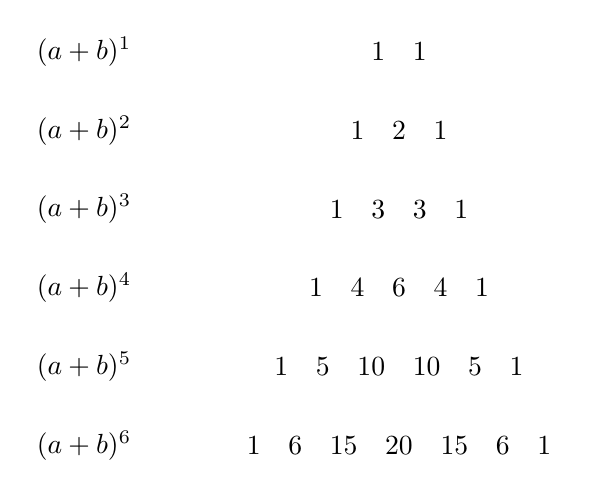
\begin{tikzpicture}
\foreach \x in {1,2,3,...,6}
{
    \node at (1,-\x){$(a+b)^{\x}$};
}
\node at (5,-1){1\quad 1};
\node at (5,-2){1\quad 2\quad 1};
\node at (5,-3){1\quad 3\quad 3\quad 1};
\node at (5,-4){1\quad 4\quad 6\quad 4\quad 1};
\node at (5,-5){1\quad 5\quad 10\quad 10\quad 5\quad 1};
\node at (5,-6){1\quad 6\quad 15\quad 20\quad 15\quad 6\quad 1};
\end{tikzpicture}
\end{center}

表中每行两端都是1，而且除1以外的每一个数都等于它肩上两个数的和。

对于二项展开式的研究，我国历史上有着极其卓越的成就。类似这样的表，宋朝数学家杨辉在所著的《详解九章算法》一书（公元1261年）中就记载了。书中提到北宋时期杰出的数学家贾宪（11世纪前期著名天文学家楚衍的学生）在研究求高次方程近似根的方法时，反复遇到两数和的任意次方的展开问题，因此，他将所发现的展开式中系数的规律造了一张数表，叫做“开方作法本源”图，载于《释锁》一书（约公元1050年，已失传），请看图7.8。这个“贾宪三角形”要比欧洲法国数学家帕斯卡（Blaise Pascal, 1623—1662年）早发现六百年。

\begin{figure}[htp]
    \centering
\begin{tikzpicture}[xscale=.7]
\node[draw, circle] at (0,6) {一};

\node[draw, circle] at (-1,5) {一};
\node[draw, circle] at (1,5) {一};

\node[draw, circle] at (-2,4) {一};
\node[draw, circle] at (0,4) {二};
\node[draw, circle] at (2,4) {一};

\node[draw, circle] at (-3,3) {一};
\node[draw, circle] at (-1,3) {三};
\node[draw, circle] at (1,3) {三};
\node[draw, circle] at (3,3) {一};

\node[draw, circle] at (-4,2) {一};
\node[draw, circle] at (-2,2) {四};
\node[draw, circle] at (0,2) {六};
\node[draw, circle] at (2,2) {四};
\node[draw, circle] at (4,2) {一};

\node[draw, circle] at (-5,1) {一};
\node[draw, circle] at (-3,1) {五};
\node[draw, circle] at (-1,1) {十};
\node[draw, circle] at (1,1) {十};
\node[draw, circle] at (3,1) {五};
\node[draw, circle] at (5,1) {一};

\node[draw, circle] at (-6,0) {一};
\node[draw, circle] at (-4,0) {六};
\node[draw, circle] at (-2,0) {\tiny 十五};
\node[draw, circle] at (0,0) {\tiny 二十};
\node[draw, circle] at (2,0) {\tiny 十五};
\node[draw, circle] at (4,0) {六};
\node[draw, circle] at (6,0) {一};

\def\x{.6}

\node[align=center]  at (-2+\x,6){本\\积};
\node[align=center]  at (-3+\x,5){商\\除};
\node[align=center]  at (-4+\x,4){平\\方};
\node[align=center]  at (-5+\x,3){立\\方};
\node [align=center] at (-6+\x,2){三\\乘};
\node[align=center]  at (-7+\x,1){四\\乘};
\node[align=center]  at (-8+\x,0){五\\乘};
\node[align=center] at (-.5,7){左\\积};
\node[align=center]  at (.5,7){右\\隅};

\draw[very thick](-8.5,-.7)--(8,-.7);

\node[align=center]   at (0,-2.5){中\\藏\\者\\皆\\廉};
\node[align=center]   at (-2,-2.5){以\\廉\\乘\\商\\方};
\node[align=center]   at (-4,-2.5){命\\实\\而\\除\\之};
\node[align=center]   at (2,-2.5){右\\袤\\乃\\偶\\算};
\node[align=center]   at (4,-2.5){左\\袤\\乃\\积\\数};
\end{tikzpicture}
    \caption{“开方作法本源”}
\end{figure}

\begin{example}
    展开$\left(3x^{3}-\frac{1}{3x^{4}}\right)^{6}$.
\end{example}

\begin{solution}
\[\begin{split}
\left(3x^{3}-\frac{1}{3x^{4}}\right)^{6}&=\comb{6}{0}\left(3x^{3}\right)^{6}+\comb{6}{1}\left(3x^{3}\right)^{5}\left(-\frac{1}{3x^{4}}\right)^{1}+\comb{6}{2}\left(3x^{3}\right)^{4}\left(-\frac{1}{3x^{4}}\right)^{2}\\
&\qquad +\comb{6}{3}\left(3x^{3}\right)^{3}\left(-\frac{1}{3x^{4}}\right)^{3}+\comb{6}{4}\left(3x^{3}\right)^{2}\left(-\frac{1}{3x^{4}}\right)^{4}\\
&\qquad +\comb{6}{5}\left(3x^{3}\right)^{1}\left(-\frac{1}{3x^{4}}\right)^{5}+\comb{6}{5}\left(-\frac{1}{3x^{4}}\right)^{6}\\
&=729x^{18}-486x^{11}+135x^{4}-20x^{-3}+\frac{5}{3}x^{-10}
-\frac{2}{27}x^{-17}+\frac{1}{729}x^{-24}
\end{split}\]
\end{solution}
 
\begin{example}
    计算$ (1+2i)^{5}$.
\end{example}

\begin{solution}
\[\begin{split}
  (1+2i)^{5}&=\comb{5}{0}+\comb{5}{1}(2i)^{1}+\comb{5}{2}(2i)^{2}+\comb{5}{3}(2i)^{3}+\comb{5}{4}(2i)^{4}+\comb{5}{5}(2i)^{5}\\
  &=61-38i
\end{split}\]
\end{solution}


从上面的例子可以看出，二项式定理给出了复数的代数形式的乘方法则，我们可以用二项式定理直接计算出复数代数形式的乘方。

\begin{example}
求$\left(2x+\frac{1}{x^{2}}\right)^{6} $中含$ x^{3} $项的系数，
\end{example}

\begin{solution}
设含$x^{3} $的项为第$( r+1 )$项，则
\[T_{r+1}=\comb{6}{r}(2x)^{6-r}\left(\frac{1}{x^{2}}\right)^{r}=\comb{6}{r}\cdot  2^{6-r}\cdot  x^{6-3r}\]

$\therefore\quad 6-3r=3\quad \implies \quad r=1$

因此，$x^{3} $的系数是$\comb{6}{1}\cdot  2^{6-1}=192$.
\end{solution}

\begin{remark}
展开式中第$( r+1 )$项的二项式系数$\comb{n}{r}$ 与第$( r+1 )$项的系数不同。在上例中$ x^{3} $项是展开式的第2项，其二项式系数是$\comb{6}{1}$, 而第二项（即含$ x^{3} $的项）的系数是$\comb{6}{2}\cdot  2^{5}=192$.    
\end{remark}

\begin{example}
    求$48^{51}$除以7的余数。
\end{example}

\begin{solution}
由于
\[\begin{split}
48^{51}&=\left(7^{2}-1\right)^{51}\\
& =\comb{51}{0}\left(7^{2}\right)^{51}+\comb{51}{1}\left(7^{2}\right)^{50}(-1)+\cdots +\comb{51}{50}\cdot  7^{2}\cdot (-1)^{50}+\comb{51}{51}(-1)^{51}\\
& =7^{102}-\comb{51}{1}\cdot  7^{100}+\cdots +\comb{51}{50}\cdot  7^{2}-1\\
&=7\left(7^{101}-\comb{51}{1}\cdot  7^{99}+\cdots+\comb{51}{50}\cdot  7^{2}-1\right)+6    
\end{split}\]

$\therefore\quad  48^{51} $除以7所得的余数为6。
\end{solution}

\begin{remark}
一个整数被7除的余数只能是$0$、$1$、$2$、$3$、$4$、 $5$、$6$中的一个。
\end{remark}

\begin{example}
    求$ 0.998^{3} $的近似值（精确到0.001）。
\end{example}

\begin{solution}
\[\begin{split}
    0.998^{3}&=(1-0.002)^{3}\\
& = 1-3\x  0.002+3\x  0.002^{2}-\cdots\\
&\approx  1-3\x  0.002\\
&=0.994
\end{split}\]
\end{solution}

\begin{remark}
    由例7.27不难看出，当$|a|$很小时， $(1+a)^{n}\approx 1+na$.
\end{remark}

\begin{example}
    求$ \left(|x|+\frac{1}{|x|}-2\right)^{3}$的常数项。
\end{example}

\begin{solution}
\textbf{解法1：}由于
\[
\left(|x|+\frac{1}{|x|}-2\right)^{3}=\left(\frac{|x|^{2}-2|x|+1}{|x|}\right)^{3}=\frac{(|x|-1)^{6}}{|x|^{3}}.\]

所以欲求的常数项应是分子的$|x|^{3}$项的系数。

而$(|x|-1)^{6} $的$ |x|^{3} $项为$\comb{6}{3}|x|^{3}(-1)^{3}=-20|x|^{3}$.

$\therefore\quad$ 展开式中的常数项为$-20$。

\textbf{解法2：}由于展开式中各项应是由$|x|$、$\frac{1}{|x|}$、$-2$所组成的因式之积。故常数项只可能由含$ |x|\cdot \frac{1}{|x|}\cdot (-2) $和$ (-2)^{3} $这样的两种形式的项构成。而$ |x|\cdot \frac{1}{|x|}\cdot (-2) $的系数是$\comb{3}{1}\comb{2}{1}(-2)$,  $(-2)^{3} $的系数是$\comb{3}{3}(-2)^{3}$. 所以常数项应为
\[\comb{3}{1}\comb{2}{1}(-2)+\comb{3}{3}(-2)^{3}=-20\]
\end{solution}

\begin{example}
    若$ \left(\sqrt{x}+\frac{1}{2\sqrt[4]{x}}\right)^{n} $展开式中前三项的系数成等差数列，求展开式中的有理项。
\end{example}

\begin{solution}
    由已知，$\comb{n}{0}+\comb{n}{2}\left(\frac{1}{2}\right)^{2}=2\left(\comb{n}{1}\cdot \frac{1}{2}\right)$,
即
\[\begin{split}
    1+\frac{1}{8}n(n-1)&=n\\
n^{2}-9n+8&=0\\
(n-8)(n-1)&=0
\end{split} \]

由题意，只有$ n=8$.
\[T_{k+1}=\comb{8}{k}\cdot  x^{\tfrac{8-k}{2}}\cdot \left(\frac{1}{2}\right)^{k}\cdot  x^{-\tfrac{k}{4}}=\comb{8}{k}\cdot \left(\frac{1}{2}\right)^{k}\cdot  x^{\tfrac{16-3k}{4}}\]

令$\frac{16-3k}{4}\in \Z$, \qquad 又$\because\quad k\in\{0,1,2,3,4,5,6,7,8\}$,

$\therefore \quad k$为0或4或8.

因此，$\left(\sqrt{x}+\frac{1}{2\sqrt[4]{x}}\right)^{8}$展开式中的有理项为
\[\begin{split}
    T_{1}&=x^{4},\\
T_{5}&=\comb{8}{4}\left(\frac{1}{2}\right)^{4}x=\frac{35}{8}x,\\
T_{9}&=\left(\frac{1}{2}\right)^{8}x^{4-6}=\frac{1}{256}x^{-2}.
\end{split}\]
\end{solution}

\begin{ex}
\begin{enumerate}
    \item 写出$ (x+2)^{7} $的展开式。
    \item 求$ (3a-2b)^{6} $展开式的第4项。
    \item 求$ \left(1+x+x^{2}\right)(1-x)^{10} $的展开式中， $x^{5} $的系数。
    \item 求$ (a+b+c)^{5} $展开式中$ ab^{3}c $的系数。
    \item 求证：$ 2^{33}+1 $是$9$的倍数。
    \item 求$ 1.002^{6} $的近似值（精确到0.001）。
    \item 设$a\ne 0$，若$ (ax+1)^{10} $和$ (x+a)^{11} $关于$x$的展开式中$ x^{5} $的系数相同，求$a$的值。
    \item 若$ \left(\sqrt{x}+\frac{1}{\sqrt[3]{x^{2}}}\right)^{n}$展开式里第五项系数与第三项系数之比为7:2，求展开式中含$x$的一次幂的项。
\end{enumerate}
\end{ex}






\section{二项式系数的性质}

我们已经知道， $(a+b)^{n} $的展开式的二项式系数是
\[
\comb{n}{0},\quad \comb{n}{1},\quad \comb{n}{2},\quad \ldots ,\quad \comb{n}{n-1},\quad \comb{n}{n}\]

观察上面所列出的展开式的二项式系数，由组合数性质
$\comb{n}{m}=\comb{n}{n-m}$，
容易发现二项式系数中，有
\[
\comb{n}{0}=\comb{n}{n},\quad \comb{n}{1}=\comb{n}{n-1},\quad \comb{n}{2}=\comb{n}{n-2},\quad \ldots ,\quad \comb{n}{k}=\comb{n}{n-k},\quad \ldots\]
即展开式的二项式系数具有正数第$k$项系数与倒数第$k$项系数相等这一性质。由此得到

\begin{thm}
{性质1} 在二项展开式中，与首末两端“等距离”的两项的二项式系数相等。    
\end{thm}


由于展开式各项的二项式系数顺次是
\[\begin{split}
\comb{n}{0}&=1,\quad \comb{n}{1}=n,\quad \comb{n}{2}=\frac{n(n-1)}{2},\quad \ldots ,\\
\comb{n}{k}&=\frac{n(n-1)(n-2)\cdots (n-k+1)}{1\cdot  2 \cdots   k},\quad \ldots ,\quad \comb{n}{n}=1.
\end{split}\]
我们可发现，后一个二项式系数的分子是前一个二项式系数分子乘以逐次减小1的数（如$n, n-1,n-2,\ldots $），分母是乘以逐次增大1的数（如$1,2,3,\ldots $），因而，各项的二项式系数从开始起是逐渐增大，又因为与首末两端“等距离”的两项的二项式系数相等，所以二项式系数增大到某一项时就会逐渐减小，且二项式系数最大的项必在中间。

当$n$是偶数时， $(n+1 )$是奇数，展开式共有 $(n+1 )$项，所以
展开式有中间一项，并且这一项的二项式系数最大。

当$n$是奇数时，$( n+1 )$是偶数，展开式共有$( n+1 )$项，所以有中间两项，这两项的二项式系数相等且最大。

由此可得到二项式系数的第二个性质。

\begin{thm}
{性质2 } 如果二项式的幂指数是偶数，中间一项的二项式系数最大；如果二项式的幂指数是奇数，中间两项的二项式系数相等并且最大。
\end{thm}

\begin{example}
    证明
\[
\comb{n}{0}+\comb{n}{1}+\comb{n}{2}+\cdots +\comb{n}{k}+\ldots +\comb{n}{n}=2^{n}\]
\end{example}

\begin{proof}
    运用$ (1+x)^{n} $的展开式
\[(1+x)^{n}=\comb{n}{0}+\comb{n}{1}x+\comb{n}{2}x^{2}+\cdots +\comb{n}{k}x^{k}+\cdots +\comb{n}{n}x^{n}\]
设$x=1$，则
\[
2^{n}=\comb{n}{0}+\comb{n}{1}+\comb{n}{2}+\ldots +\comb{n}{k}+\cdots +\comb{n}{n}\]
\end{proof}


例7.30说明，$ (a+b)^{n} $的展开式的所有二项式系数的和等于$ 2^{n}$. 这是一个重要的结论。

\begin{example}
   证明在$ (a+b)^{n} $的展开式中，奇数项的二项式系数的和等于偶数项的二项式系数的和。 
\end{example}

\begin{proof}
    在展开式
\[(a+b)^{n}=\comb{n}{0}a^{n}+\comb{n}{1}a^{n-1}b+\comb{n}{2}a^{n-2}b+\cdots +\comb{n}{n}b^{n}\]
中，设$ a=1$, $ b=-1$，得
\[(1-1)^{n}=\comb{n}{0}-\comb{n}{1}+\comb{n}{2}-\comb{n}{3}+\cdots +(-1)^{n}\comb{n}{n}\]
就有
\[
0=\left(\comb{n}{0}+\comb{n}{2}+\cdots \right)-\left(\comb{n}{1}+\comb{n}{3}+\cdots \right)\]

$\therefore\quad \comb{n}{0}+\comb{n}{2}+\cdots =\comb{n}{1}+\comb{n}{3}+\cdots$

即$(a+b)^{n} $的展开式中，奇数项的二项式系数的和等于偶数项的二项式系数的和。
\end{proof}

以上两例实际上用到了二项式定理是一个恒等式这一事实。由于恒等式对于式中字母允许取的任意数值，两边均相等。所以在例7.30中我们取$x=1$; 例7.31中取$ a=1$,  $b=-1$, 这样就可得到二项式系数和的性质。

\begin{example}
    求证：
\[ 1-\comb{40}{2}+\comb{40}{4}-\comb{40}{6}+\comb{40}{8}-\comb{40}{10}+\cdots +\comb{40}{40}=2^{20}\]
\end{example}

\begin{proof}
    在$ (a+b)^{40} $的展开式中，令$ a=1$, $b=i$, 则
\[\begin{split}
    (1+i)^{40} &=\left(1-\comb{40}{2}+\comb{40}{4}-\comb{40}{6}+\cdots +\comb{40}{40}\right)\\
    &\qquad +i\left(\comb{40}{1}-\comb{40}{3}+\comb{40}{5}-\comb{40}{7}+\cdots-\comb{40}{39}\right)
\end{split}
\]

又$\because\quad (1+i)^{40}=\left[(1+i)^{2}\right]^{20}=(2i)^{20}=2^{20}$,

$\therefore\quad 1-\comb{40}{2}+\comb{40}{4}-\comb{40}{6}+\cdots +\comb{40}{40}=2^{20}$.
\end{proof}

\begin{remark}
\begin{enumerate}
    \item 由例7.32的证明还可得出
\[\comb{40}{1}-\comb{40}{8}+\comb{40}{5}-\comb{40}{7}+\cdots -\comb{40}{39}=0\]
\item 此题的结论可推广到一般的情形
\[\begin{split}
    \comb{n}{0}-\comb{n}{2}+\comb{n}{4}-\comb{n}{6}+\cdots  &=(\sqrt{2})^{n}\cos\frac{n\pi }{4};\\
\comb{n}{1}-\comb{n}{3}+\comb{n}{6}-\comb{n}{7}+\cdots &=(\sqrt{2})^{n}\sin\frac{n\pi }{4}.
\end{split}\]
\end{enumerate}
（请读者自己证明）
\end{remark}

作为多项式恒等式（二项展开式就是其中之一）有一个很重要的性质，就是恒等式左、右两端的对应项系数相等。利用这一性质，我们同样可以求得一些有关组合数之间的关系式。

\begin{example}
    求证： $\comb{3}{3}+\comb{4}{3}+\comb{5}{3}+\cdots +\comb{100}{3}=\comb{101}{4}$.
\end{example}

\begin{proof}
$\comb{3}{3}+\comb{4}{3}+\comb{5}{3}+\cdots +\comb{100}{3} $可看成$ (1+x)^{3}+(1+x)^{4} +(1+x)^{5}+\cdots +(1+x)^{100} $展开式中含$ x^{3} $项的系数。

\[\begin{split}
    \text{又}\because &\quad (1+x)^{3}+(1+x)^{4}+(1+x)^{5}+\cdots +(1+x)^{100}\\
&=\frac{(1+x)^{3}[(1+x)^{98}-1]}{(1+x)-1}\\
&=\frac{(1+x)^{101}-(1+x)^{3}}{x}
\end{split}\]

$\therefore\quad$ 展开式中含$ x^{3} $项的系数又应为$ \comb{101}{4}$,

$\therefore\quad \comb{3}{3}+\comb{4}{3}+\comb{5}{3}+\cdots +\comb{100}{3}=\comb{101}{4}$.
\end{proof}

\begin{ex}
\begin{enumerate}
    \item 填空
\begin{enumerate}[(1)]
 \item $(x+y)^{2n}\; (n\in \N) $的展开式中，系数最大项是第$\underline{\qquad\qquad}$项。
   \item $(1-x)^{95}$展开式中系数最小的项是$\underline{\qquad\qquad}$.
   \item $\comb{n}{1}+\comb{n}{2}+\comb{n}{8}+\cdots +\comb{n}{n-1} $的值是  $\underline{\qquad\qquad}$.
   \item 
若$ (a+b)^{n} $展开式中偶数项的系数之和等于256，则$n$为$\underline{\qquad\qquad}$.
   \item 
若$ \comb{19}{n} $与$ \comb{n}{m} $同时有最大值，则$m$为$\underline{\qquad\qquad}$.
   \item 
$\left(x^{2}-\frac{1}{2y}\right)^{10} $展开式的所有项系数之和是$\underline{\qquad\qquad}$. 
\end{enumerate}
\item 化简$ 1+2\comb{n}{1}+4\comb{n}{2}+\cdots +2^{k-1}\comb{n}{k-1}+\cdots +2^{n}\comb{n}{n}$.

\item 求$ (1+x)+(1+x)^{2}+\cdots +(1+x)^{n} $的展开式中各项系数之和。
\end{enumerate}
\end{ex}




\section*{习题四}
\begin{center}
\bfseries A
\end{center}

\begin{enumerate}
    \item 用二项式定理展开：
\begin{enumerate}[(1)]
    \item $(a+\sqrt[3]{b})^{9}$;
 \item $\left(\frac{\sqrt{x}}{2}-\frac{2}{\sqrt{x}}\right)^{7}$.
\end{enumerate}

\item 求 $\left(x^{3}+2x\right)^{7}$ 的展开式的第4项的二项式系数，并求第4项的系数。
\item 求 $(x+y+z)^{6}$ 的展开式中，含 $x^{3}y^{2}z$ 项的系数。
\item 化简：
\begin{enumerate}[(1)]
 \item $(1+\sqrt{x})^{5}+(1-\sqrt{x})^{5}$;
 \item $\left(2x^{\tfrac{1}{2}}+3x^{-\tfrac{1}{2}}\right)^{4}-\left(2x^{\tfrac{1}{2}}-3x^{-\tfrac{1}{2}}\right)^{4}$.
\end{enumerate}

\item \begin{enumerate}[(1)]
    \item 求$ (1-2x)^{15} $的展开式中前4项；
    \item 求$ \left(2a^{3}-3b^{2}\right)^{10} $的展开式中第8项；
    \item 求$ \left(\frac{\sqrt{x}}{3}+\frac{3}{\sqrt{x}}\right)^{12}$ 的展开式的中间一项；
    \item 求$ (x\sqrt{y}-y\sqrt{x})^{15} $的展开式的中间两项。
\end{enumerate}

\item 求下列各式的二项展开式中指定各项的系数：
\begin{enumerate}[(1)]
    \item $\left(\sqrt{x}+\frac{1}{x^{2}}\right)^{10} $的展开式中不含$x$的项；
    \item $\left(1-\frac{1}{2x}\right)^{10}$ 的含$ \frac{1}{x^{5}}$ 的项。
\end{enumerate}

\item 
求下列各数的近似值（精确到0.001）:
\begin{multicols}{2}
\begin{enumerate}[(1)]
    \item $(1.003)^{5}$;
    \item $(0.9998)^{8}$.
\end{enumerate}
\end{multicols}

 \item 在$ (ax+1)^{7} $的展开式中，$ x^{3} $的系数是$ x^{2} $的系数与$ x^{4} $的系数的等差中项，若实数$ a>1$，求$a$的值。

 \item 若$(1-2x)^{5} $的展开式中，$T_{2}>T_{1} $且$T_{2}\ge T_{3}$，求$x$的取值范围。

 \item 用二项式定理证明：
\begin{enumerate}[(1)]
    \item $(n+1)^{n}-1$ 能被$n^{2}$ 整除；
    \item $99^{10}-1$ 能被1000整除。
\end{enumerate}

\item 求证：
\begin{enumerate}[(1)]
 \item $2^{n}-\comb{n}{1}2^{n-1}+\comb{n}{2}2^{n-2}+\cdots +(-1)^{n-1}\comb{n }{n-1}\cdot  2+(-1)^{n}=1$;
   \item $8^{n}+8^{n-1}\comb{n}{1}+8^{n-2}\cdot  \comb{n }{2}+\ldots +8\comb{n}{n-1}+\comb{n}{n}=3^{2n}$. 
\end{enumerate}
\end{enumerate}


\begin{center}
    \bfseries B
\end{center}

\begin{enumerate}
 \setcounter{enumi}{11}  
  \item 证明：
  \begin{enumerate}[(1)]
    \item $\left(x-\frac{1}{x}\right)^{2n} $的展开式中常数项是
\[(-2)^{n}\frac{1\cdot  3\cdot  5\cdots (2n-1)}{n!}\]
\item $(1+x)^{2n}$ 的展开式的中间一项是
\[\frac{1\cdot  3\cdot  5\cdots (2n-1)}{n!}(2x)^{n}\]
\end{enumerate}

\item 求证：$ 3^{3n}-26n-1 $能被676整除。
\item 若$ (63x+10y)^{73} $展开式中各项系数之和为$A$, $(63x- 10y)^{53}$ 展开式中各项系数之和为$B$，求证：$ (A-B) $能被10整除。

\item 已知$ \left(1+x^{2}\right)+\left(1+x^{2}\right)^{2}+\left(1+x^{2}\right)^{3}+\cdots +\left(1+x^{2}\right)^{20}$,
\begin{enumerate}[(1)]
   \item 求展开式中$ x^{4} $的系数；
  \item 求展开式中各项系数之和。
\end{enumerate}
\item 在 $\left(x^{3}+x^{-2}\right)^{n}\quad (n\in N)$ 展开式中，若存在常数项，求$n$
的最小值。

\item 若$(\sqrt[3]{2}x-\sqrt{2^{-1}})^{n} $展开式中的末项绝对值为 $\left(\frac{1}{3\sqrt[3]{9}}\right)^{\log_{3}{8}}$，求展开式的第五项。
\end{enumerate}




\section{本章小结}

\subsection*{（一）知识结构}

\begin{center}

\begin{tikzpicture}[>=stealth]
\node[draw](A) at (0,-.25) {基本原理}; 
\node[draw](B1) at (3,.5) {排列与排列数公式};
\node[draw](B2) at (3,-1) {组合与组合数公式};
\node[draw](B3) at (3,-2.5){二项式定理};
\node[draw](C1) at (7,-1){组合数的两个性质};
\node[draw](C2) at (7,-2.5){二项式系数的性质};
\draw[->](B1)--(B2);
\draw[->](B2)--(B3);
\draw[->](B2)--(C1);
\draw[->](B3)--(C2);
\draw[decorate, decoration={brace, amplitude=5pt}](1.2,-1)--(1.2,.5);

\end{tikzpicture}
\end{center}


\subsection*{（二）几点说明}
\begin{enumerate}
    \item 加法原理和乘法原理是两个基本原理，它们不仅是推导排列数公式、组合数公式的基础，而且可用它们直接去解决某些问题。要正确地使用它们，首先就要弄清在所遇到的问题中，“做一件事”是指什么。
    \item 弄清排列和组合这两个概念，注意它们的区别和联系。这种区别和联系的数量形式就是排列数公式与组合数公式的区别和联系。
    \item 本章的主要公式是：

    排列数公式
\[\begin{split}
 \perm{n}{m}&=n(n-1)(n-2)…(n-m+1)=\frac{n!}{(n-m)!}\quad (m\le n);\\
\perm{n}{n}&=n!=n(n-1)(n-2)\cdots 2\cdot 1   
\end{split}\]

组合数公式
\[
\comb{n}{m}=\frac{n(n-1)(n-2)…(n-m+1)}{1\cdot 2\cdots m}=\frac{n!}{(n-m)!m!}\quad (m\le n)\]

组合数性质
\[\begin{split}
    \comb{n}{m}&=\comb{n}{n-m}\quad (m\le n)\\
\comb{n+1}{m}&=\comb{n}{m}+\comb{n}{m-1}\quad (m\le n)
\end{split}\]

二项式定理
\[
(a+b)^{n}=\comb{n}{0}a^{n}+\comb{n}{1}a^{n-1}b+\cdots+\comb{n}{r}a^{n-r}b^{r}+\cdots+ \comb{n}{n}b^{n}\]

二项展开式的通项，即第$( r+1 )$项
\[
T_{r+1}=\comb{n}{r}a^{n-r}b^{r}\]


二项式系数的主要性质
\begin{enumerate}[(1)]
 \item 在二项展开式中，与首末两端“等距离”的两项的二项式系数相等。
 \item 如果二项式的幂指数是偶数，中间一项的二项式系数最大；如果二项式的幂指数是奇数，中间两项的二项式系数相等并且最大。   
\end{enumerate}


\item 加法原理，乘法原理和上述所有公式都是数学模型。灵活应用它们解决问题的关键是对所给问题的分析及对模型的深刻理解。用映射的观点处理排列问题会更加清晰。
\end{enumerate}



\section*{复习题七}
\begin{center}
    \bfseries A
\end{center}

\begin{enumerate}
    \item 求证
\begin{enumerate}[(1)]
    \item $\frac{(2n)!}{2^{n}\cdot  n!}=1\cdot  3\cdot  5\cdot \cdots \cdot (2n-1)$;
    \item $\frac{1}{2!}+\frac{2}{3!}+\cdots +\frac{n}{(n+1)!}=1-\frac{1}{(n+1)!}$.
\end{enumerate}

\item 解方程：
\begin{enumerate}[(1)]
    \item $3\comb{x-3}{x-7}=5\perm{x-4}{2}$;
    \item $\frac{\perm{n}{4}+\perm{n}{3}}{\comb{n}{2}}=50$.
\end{enumerate}


\item 四个学生分配到三个车间去劳动，有多少种分配方法？三个学生分配到四个车间呢？

\item 求证：
\[
\comb{n}{1}+2\comb{n}{2}+3\comb{n}{8}+\cdots +n\comb{n}{n}=n\cdot  2^{n-1}\]

\item 从$0,1,2,3,4,5$六个数字中：
\begin{enumerate}[(1)]
    \item 任取三个不同数字编号码，能编几种不同的号码？
    \item 如果任取三个不同的数字，组成三位数，有多少种不同的三位数？
    \item 如果任取三个数字做电话号码（数字可重复），有多少种不同的电话号码？
    \item 如果任取三个不同的数字，可组成多少个不同的偶数？
\end{enumerate}

 \item 用1、2、3、4、5，这五个数字可组成比30000大，并且百位数字不是3的没有重复数字的五位数有多少个？
 \item 
有八个人站在一横排，其中甲、乙、丙三人相邻的排法有多少种？甲、乙、丙三人互不相邻的排法有多少种？
 \item 七人一排照相，其中一人不排在两端，也不排在正中间，共有多少种不同的排法？

 \item 五男五女排成一排。
\begin{enumerate}[(1)]
    \item 其中五男排在一起的排法有多少种？
    \item 其中男女相间的排法有多少种？
    \item 其中五男不能相邻的排法有多少种？
    \item 其中五男必须按从高到矮的顺序的排法有多少种？
\end{enumerate}
    \item 已知复数$ x+yi$，如果$x$、$y$可分别取$0,1,2,3,\ldots, 9$这十个数字中的任何一个，可以组成多少个复数？可以组成多少个虚数？
    \item 有六名短跑运动员，选出其中四人参加竞赛。
\begin{enumerate}[(1)]
    \item 必须甲参加的有多少种选法？
    \item 乙不能参加的有多少种选法？
\end{enumerate}
 \item 从6名男生和4名女生中，选出5名学生观看演出，要求其中至少要有2名男生和1名女生，问有多少种不同的选法？

 \item 从14名工人中选出5人，分配到6台不同性质的机床上工作（每台至多分配1人），问有多少种不同的分配方法？

 \item 八名男生和五名女生中，选出5人来排队，若奇数位置上必须是女生，问有多少种不同的排法？
 \item 已知$\left(\sqrt{x}+\frac{1}{x^{2}}\right)^{n} $的展开式中，第5项的系数与第3项的系数的比是14:3，求展开式中的常数项。

 \item 若$\left(\sqrt[3]{x}-\frac{2}{x}\right)^{n} $展开式中第八项是含$ \sqrt[3]{x} $的项，求展开式中$ \frac{1}{x} $项是第几项。
\end{enumerate}

\begin{center}
\bfseries B
\end{center}

\begin{enumerate}
\setcounter{enumi}{16} 
  \item 从$1,2,\ldots,10$这十个数中取出四个数，使它们的和为奇数，共有多少种取法。
  \item 
将数字$1,2,3,4$填入标号为$1,2,3,4$的四个方格里，每格填一个数字，并使每个方格的标号与所填数字均不相同，共有多少种填法。
  \item 
11名工人中5人只会排版，4人只会印刷，另2人既会排版也会印刷，现从中选出4人排版、4人印刷，共有多少种选法？
  \item 
由$0,1,2,\ldots,9$这十个数字组成六位数，且要求其中含有三个5，其他无重复数字，问这样的六位数有多少个？

  \item 平面内有9条直线。
\begin{enumerate}[(1)]
    \item 如果其中没有互相平行的直线，也没有三条以上交于一点的直线，问可构成多少个不同的三角形？
    \item 如果其中有4条互相平行，没有三条相交于一点的，问可构成多少个不同的三角形？
    \item 如果其中没有相互平行的直线，而且只有四条交于一点的，问可构成多少个不同的三角形？
\end{enumerate}

\item 任取圆周上15个点，每两点连一条弦，求所有的弦在圆内的交点最多有多少个？
\item \begin{enumerate}[(1)]
    \item 求$ 1988^{1989} $除以9所得的余数；
    \item 证明：当$ n\in \N $时， $3^{2n+2}-8n-9 $能被64整除。
\end{enumerate}

\item 如果$a_{1},a_{2},a_{3},a_{4}$ 为二项展开式中的相邻四项的二项式系数，求证：
$\frac{a_{1}}{a_{1}+a_{2}}$, $\frac{a_{2}}{a_{2}+a_{3}}$, $\frac{a_{3}}{a_{3}+a_{4}}$ 成等差数列。
\end{enumerate}

\begin{center}
\bfseries C
\end{center}

\begin{enumerate}
  \setcounter{enumi}{24}  
  \item 八个人分两排坐，每排4人，限定甲必须坐在前排，乙、丙必须坐在同一排且相邻，共有多少种不同坐法？
  \item $A,B,C,\ldots$等七人排成一排，若$A$、$B$均不与$C$相邻，共有多少种不同的排法？
\item 若$(3x-1)^{7}=a_{0}x^{7}+a_{1}x^{6}+a_{2}x^{5}+\cdots+a_{6}x+a_{7}$.
\begin{enumerate}[(1)]
    \item 求$ a_{0}+a_{1}+a_{2}+\cdots+a_{7} $的值；
    \item 求$ a_{0}+a_{2}+a_{4}+a_{6}$ 和$ a_{1}+a_{3}+a_{5}+a_{7} $两式的值。
\end{enumerate}

\item 证明：
\[
\comb{n}{0}\comb{n+2}{3}+\comb{n}{1}\comb{n+2}{4}+\comb{n}{2}\comb{n+2}{5}+\cdots+\comb{n}{n-1}\comb{n+2}{n+2} =\comb{2n+2}{n+3}\]

\item 求$\left(1+x+\frac{1}{x^{3}}\right)^{7}$ 展开式中的常数项。

\item 利用二项式定理证明：$\frac{48}{47}\left(48^{8}-1\right)$是能被7整除的自然数。
\item 在$ (a+b)^{n} $的展开式中，若前后相连接的三项的系数依次为20、15、6，求$n$及这三个系数所在的项数。

\item 求$ (3x-2y+2)^{5} $展开式中含$x^{2}yz^{2}$ 项的系数。
\end{enumerate}

